\documentclass{report}
\usepackage[utf8]{inputenc}
\usepackage{xcolor}
\usepackage{url}
\usepackage[nottoc]{tocbibind}
\usepackage{graphicx}
\usepackage[bottom]{footmisc}
\usepackage{cite}
 

\title{Project Document: Deep(FAMS)}
\author{Mohammad Alyetama \\
Ali Al-Ramini \\
Fangyi Li }
\date{}

\begin{document}

\maketitle

\tableofcontents

\begin{abstract}
This is the template you are required to use for your project milestone write-ups.  Each submission will build on the previous one.  At this spot in your report, you should place a brief abstract (4--6 sentences). This is a high-level summary of your work, including a brief summary of the problem, motivation, and your results.  Since your work will evolve for each milestone, the abstract should get updated with each submission.
\end{abstract}

\chapter{Milestone 1: Project Ideas}

\section{Introduction}

\subsection{Project Idea 1}
Here you should give an 
overview of your process, where you looked for project ideas. Citations are important. 

A few other notes, since I have your attention. First, you should be using figures and/or tables, especially in later milestones with experimental results.  If you have no tables or figures to summarize experimental results, then something is very, very wrong. 

Second, you {\bf must} refer to your figures and tables in the main text, and summarize/explain each of  them.  Each figure/table {\bf must have a caption}.  Table captions go {\bf above} the table, and figure captions go {\bf below} the figure\footnote{I don't make the rules, but I will enforce them.}. 

For example, Figure~\ref{fig:compute} shows how computing power requirements for cutting-edge deep learning projects have increased over time. At this point, we would maybe point out a few interesting things, like how quickly it increases after 2011. Then, for a completely unrelated note in the same paragraph\footnote{Don't do this!}, Table~\ref{tab:CNN-perf} summarizes  performance of various CNN architectures on ImageNet.  Here we could point out how quickly the error rates drop. 

\begin{figure}
    \centering
    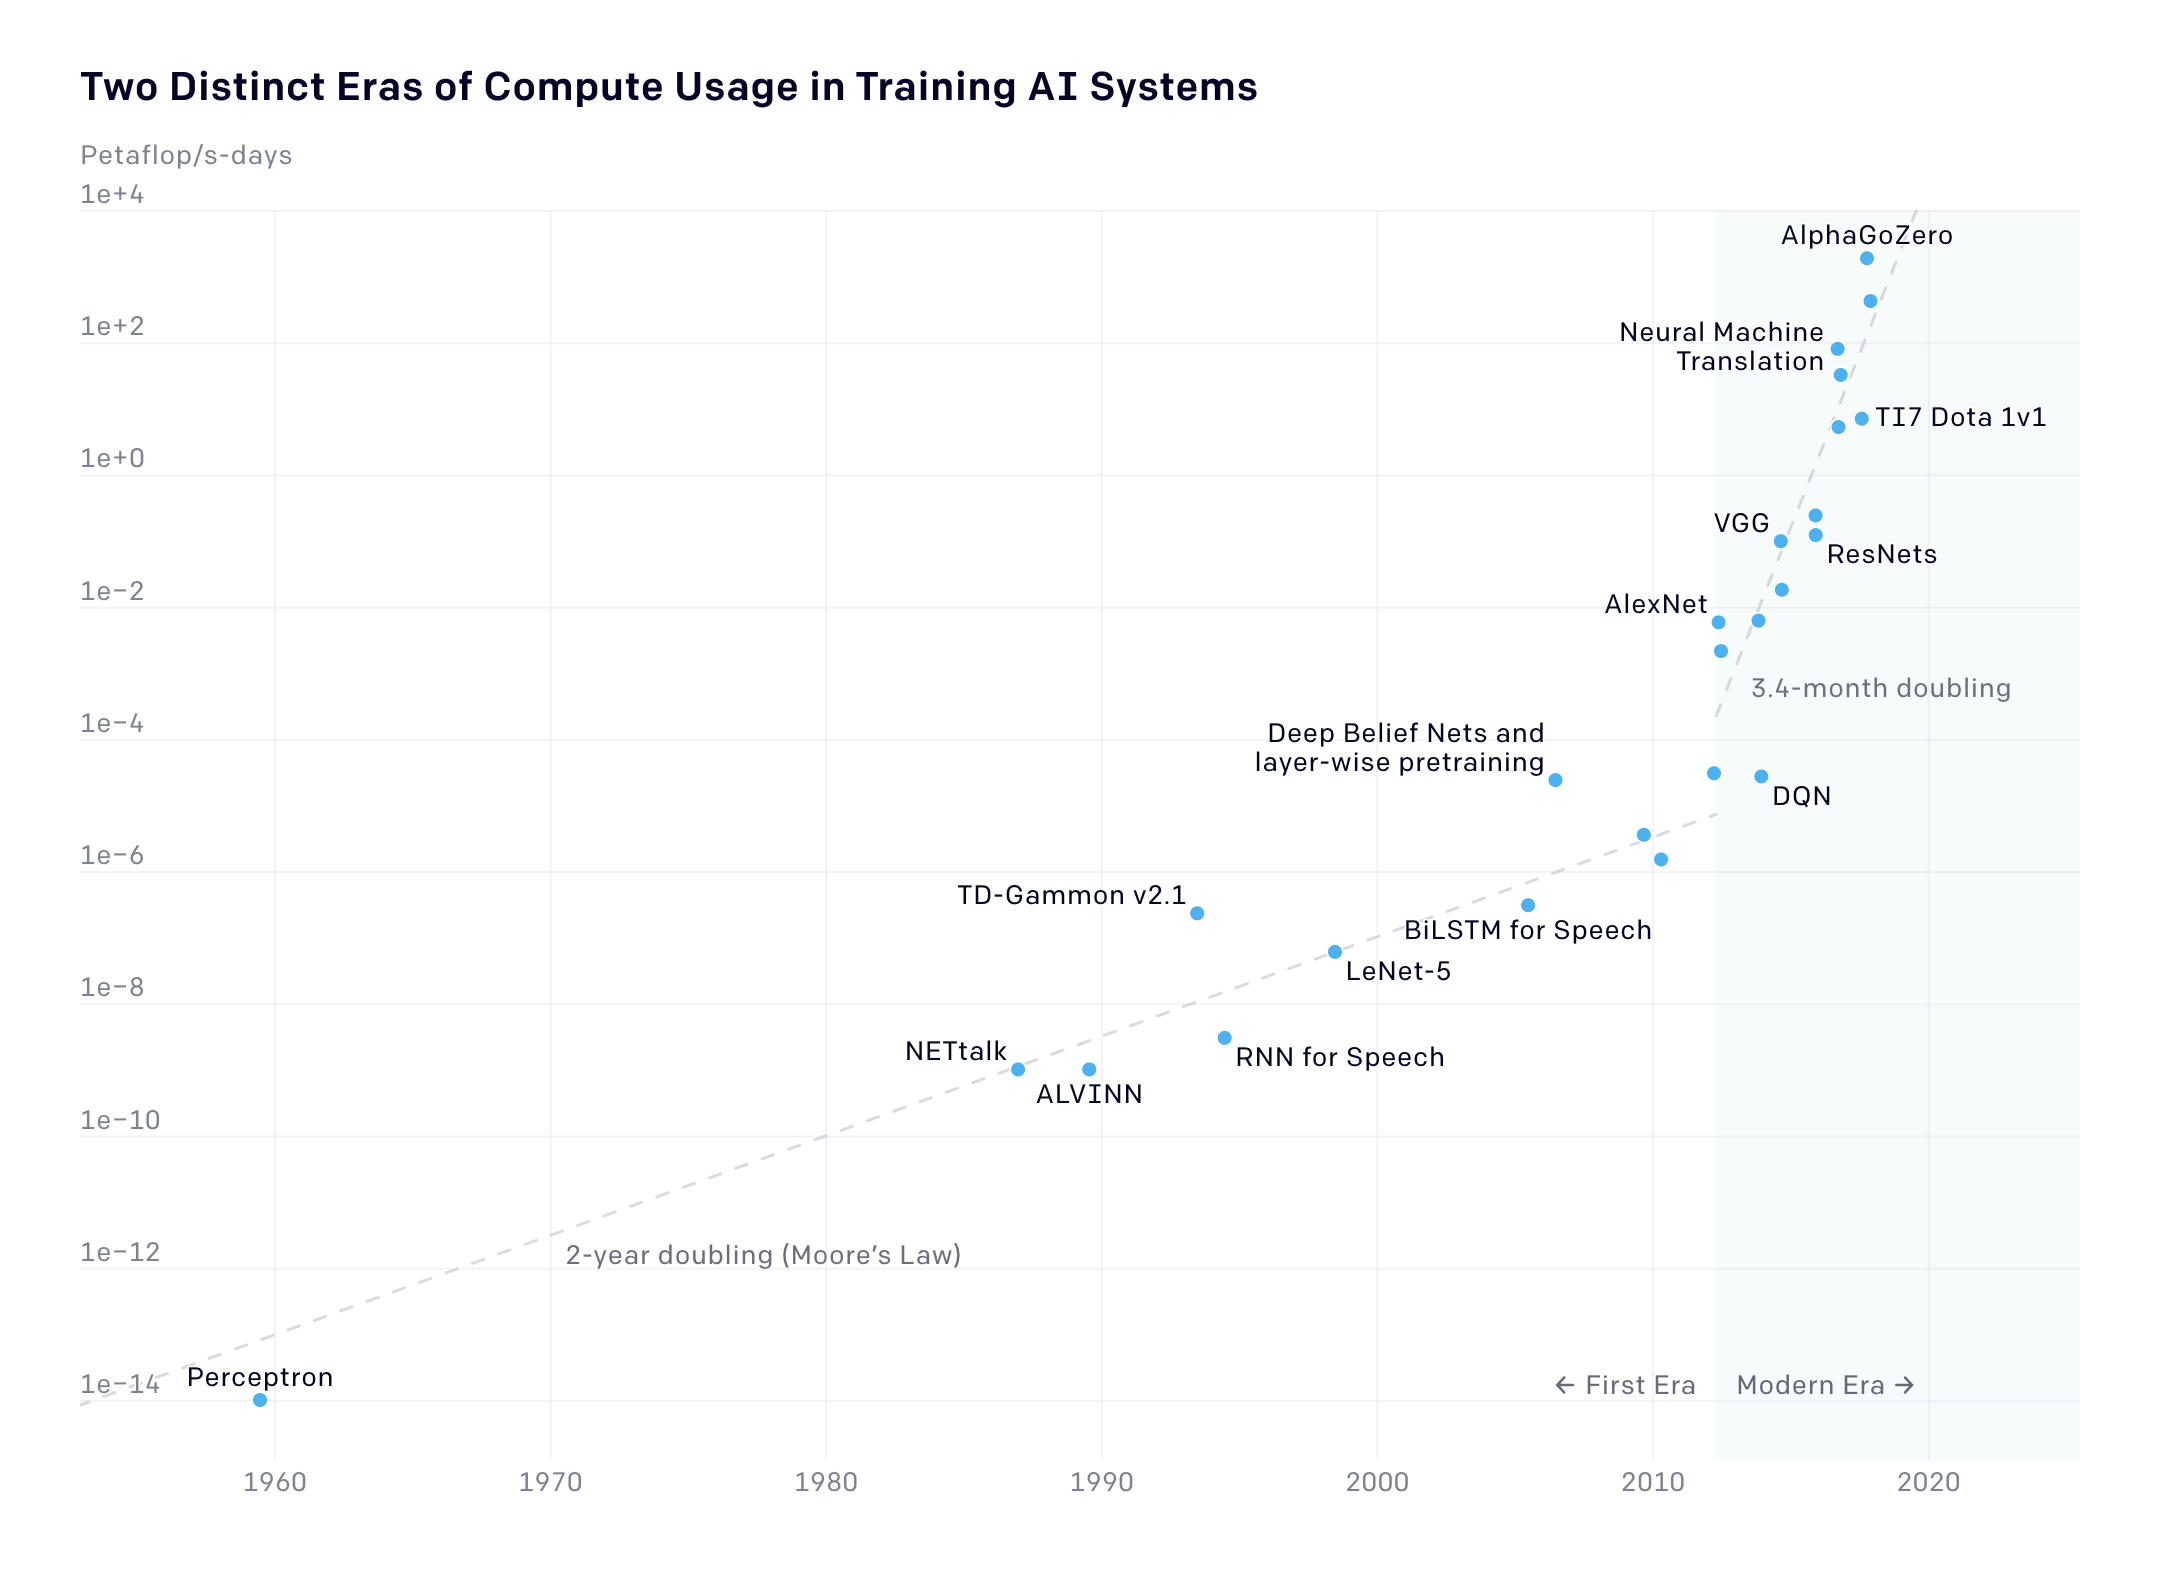
\includegraphics[width=\textwidth]{figs/ai-and-compute-all-2.png}
    \caption{Compute for cutting-edge deep learning projects vs.\ time (source:~\cite{AI-compute18}).}
    \label{fig:compute}
\end{figure}

\begin{table}[]
    \centering \caption{Top-5 error on ImageNet for various convolutional architectures.}
    \begin{tabular}{|c|c|c|} \hline
      Architecture   &  Year & Top-5 Error \\ \hline
    AlexNet & 2012     & 17\% \\
    GoogLeNet & 2014 & 7\% \\
    ResNet & 2015 & 3.6\% \\ \hline
    \end{tabular}
 
    \label{tab:CNN-perf}
\end{table}

\subsection{Project Idea 2}
There is a great interest in improving the cycling infrastructure in Nebraska by analyzing cyclic data. Toward this goal, we acquired the Strava Metro data that covers the state of Nebraska from January 2017 to December 2019.  Strava provides data into four categories edges, nodes, origin-destination polygons, and shapefiles that contain spatial attributes to create maps using GIS software. Edges are street segments between nodes. In other words, a set of edges form a street. Nodes are the intersections between edges, and origin-destination polygons divide a space into smaller areas. Every category of Strava data is divided into yearly, monthly, and hourly data. The Strava data, made available by the social fitness network company Strava, includes raw data for the hour-by-hour counts for bicycle trips that have been mostly incorporated into existing maps for better visualization. In this project, we propose building a deep learning regression model that utilizes Strava data in addition to weather data to predict the number of cycling trips in Nebraska. 



\section{Project Idea 1: Evaluating the Reproducibility of Training GAN With Limited Data}

Generative adversarial networks (GAN) is a generative modeling approach that uses deep learning techniques to automatically discover and learn the patterns in the input to generate an output that would plausibly appear as if it was sampled from the original input data. For example, a GAN that uses convolutional neural networks (CNNs) can take photographs of humans as its input data and generate new photographs of humans with plausible characteristics that looks superficially genuine. This approach gained popularity after it was introduced for the first time by Goodfellow et al. <CITE>. In their paper, they describe GAN as a structure with two essential sub-models: (1) a generator model that learns to generate superficially plausible data, which the discriminator takes as a negative training examples, and (2) a discriminator model that learns to discriminate between generated and real data, and penalizes the generator if an implausible result is detected. Here, the generator and the discriminator are neural networks that are directly connected. This connection allows the discriminator to send a signal, through backpropagation, that the generator uses to update its weights. Specifically, the generator samples a vector that is randomly drawn from a Gaussian distribution and use it to seed its generative process and match it to a distribution of interest, creating a "latent space." With sufficient training, the generator model can learn the statistical latent space of the input data and create output data similar to what is observed in the input data. An example of such data is then processed by the discriminator model and attempt to distinguish it from the real distribution of the data (i.e., a binary class of fake/real). The generator model's goal here is to maximize the error of the discriminator model. In other words, the generator model becomes more effective the more the discriminator process fake data as real data. The GAN approach has been used in fashion, science and video games with impressive results <source>.

A major challenge in this area, however, is the large number of data required to build a good GAN model, which is in some cases not available for researchers interested in applying GAN to their research question. The reason why GAN typically requires a large dataset is because with smaller datasets, the discriminator model ends up overfitting to training data examples and the training eventually diverge. While dataset augmentation is typically applies in such situations to solve the problem of overfitting, this cannot be achieved in GAN models. The inability of solving this problem with dataset augmentation stems from the ability of GAN in employing this technique without learning the augmented distribution and leaking this results to the model, causing an undesirable outcome <SOURCE>. Therefore, the challenge is to demonstrate that GAN can be used with smaller datasets without the aforementioned pitfalls.

A recent attempt to solve this problem was proposed by Kerras et al., demonstrating that it is possible to obtain good results using limited data. The key point in their proposed approach is that the issue of overfitting and augmentations leak can be prevented by applying a wide variety of augmentation methods. In their work, they demonstrate the validity of their approach by describing a set of conditions that allows to control the augmentations leak problem, then propose an adaptive discriminator augmentation pipeline that is able to dynamically control the strength of the augmentation. This is a novel approach they propose contrasting the convention of tuning the augmentation strength manually, a resources-consuming process. The process of building an adaptive discriminator augmentation mechanism, as described by the authors, is achieved by 
(a) Declare an overfitting heuristic, r, in which a value of zero represents no overfitting and a value of 1 means perfect overfitting <EQUATION 1>.
(b) Adjust augmentation probability (p) until the heuristic reaches a target value, which in turn can be processed by:
(1) initializing the augmentation strength to zero, then adjusting p every 4 minibatches based on an overfitting heuristic (rf).
(2) if rf shows too much overfitting, it is countered by a fixed increment of p (or fixed decrement if rf shows too little overfitting).
(3) The adjustment size is then set in a way that allows p to quickly rise from 0 to 1, while clamping p after every step from below to zero (adaptive).
(4) The results from adaptive versus fixed p are then compared.
By using such mechanisms on limited data, the authors demonstrated that their adaptive discriminator augmentation approach was able to improve the results quality and stabilize training with a minimal effect on resources consumption, showing that their approach is both viable and cost-efficient.


In this project, we attempt to reproduce a proposed solution by Karras et al. to this problem. 



\section{Project Idea 2: Using App Data to Model Bicycling Patterns in Nebraska}

Across the United States, cycling is becoming increasingly popular as users shift travel modes amid concerns of health, physical activity, air, and environmental quality, and to escape roadway congestion. Unfortunately, the infrastructure in the U.S. traditionally caters to automobile traffic creating impediments for bikers and impacting their safety. To accommodate cycling, a major challenge is the lack of machine learning model representation of the available data to assess the attributes of present assets accurately and to inform additional investments to integrate bicycles into our transportation system. Toward that end, this project uses citywide bicycle travel data (i.e., Strava Metro Data) to provide a comprehensive description of daily cycling in a mid-size American state, as a proof-of-concept approach to planning for cycling. 
\\Various governments and organizations are utilizing big data to evaluate their cycling infrastructure ~\cite{hall2012open}. Big cycling data are usually collected using live point data, journey data, Bike-Share Programs (BSP), and GPS. Live point data are collected on intersections using cameras on traffic lights, counting stations, or even sensors. While the journey data provide information about the origin and the destination of the trip, it does not provide the details of the trip. This set of data could be collected from BSP or by other sources like online questionnaires. BSP data are complete and in real-time. However, these data only give information within the area of its location ~\cite{ romanillos2016big, rogers2000counting}. Strava considered a GPS program that is made available by the social fitness network company Strava. Strava utilizes the Open Street Map (OSM) to deliver its data. These GPS data are very detailed and historical but represent a small sample of the total population of the cyclists.  
Strava app data contains a vast amount of spatial and temporal details to predict cycling activities pattern. It provides a good approximation of the most-used routes and the peak months and hours. To protect privacy, the Strava data set is combined into population datasets. While a small portion of cyclic may use Strava to log their trips or the app might track trips for users using other transportation methods ~\cite{hall2012open, romanillos2016big, fishman2016cycling }, several studies showed that there is a strong correlation between the Strava data, and the ground-truth data obtained from counting stations ~\cite{hong2020evaluation, jestico2016mapping}. 
Cycling is affected by several factors such as weather, time of the day, infrastructure, congestion, environment, income, public transportation, health, population density, the slope of the street, and cultural view towards cycling ~\cite{musakwa2016mapping, roy2019correcting, hochmair2019estimating} . But traditionally access to high-quality data has limited our understanding of cycling behavior and route choice in the face of these myriad factors. In this project, we explore the weather effects and weather parameters sensitivity to cycling in Nebraska. The goal of this work is to further specify cycling behavior as it relates to specific factors, but more importantly, to determine the quality of the specified factors in determining the number of cycling trips over a huge area like the State of Nebraska. 
Using data visualization techniques and Deep learning regression (e.g., ANN, RNN, LSTM, and GRU)~\cite{hassoun1995fundamentals, graves2013generating} we study the most influential time-related factors affecting the cycling patterns in Nebraska. Moreover, cycling is usually categorized into two classes, commuting and recreational. The proposed study will take advantage of the data shared by Strava to predict the number of commute and recreational activities across all streets. 

 

\section{Conclusions}
\subsection{Project Idea 1}
Sum up your results, including your opinion on each project idea.  Also, list any questions that you have for the instructor and TA regarding your project work.

\textcolor{red}{Remember to cite sources using BiBTeX and add those references to the end of this document!}

It is okay to cite some websites and tutorials (if you first look up how to properly cite them!), but you must also cite some refereed publications from conferences and/or journals.

Sample citation~\cite{Samuel59}

\subsection{Project Idea 2}
This project provides an interesting idea, which is to create a deep learning model that predicts the cycling patterns in Nebraska. With the help of high-quality data sources (e.g., Strava Data and Weather Data) the outcomes of this project could be very important towards understanding how cyclists react to temporal variations. However, the spatial factors affecting cycling should be also studied adding more complexity to the problem. The spatial representation of the data could be very hard to map during this short period of time. 


\appendix

\chapter{First Appendix}

An appendix is used only if necessary (remove this chapter if you don't use one). It contains supplementary materials/extra details such as extensive experimental results (e.g., hyperparameter search results, where the most interesting ones are in the main text and the rest are dumped here), detailed proofs, etc. 

Create as many appendices as needed by adding chapters. All such chapters must be before the bibliography. 


\bibliographystyle{plainurl}
\bibliography{main}

\end{document}
